\chapter{Livesignage su WebOS}\label{svolgimento}
\section{In Breve}
Descrizione del lavoro svolto: \edit{portare l'applicazione già esistente per i dispositivi Samsung sui dispositivi LG}, difficoltà incontrate e soluzioni trovate, modifiche all'applicazione pre-esistente. Descrizione della fase di testing finale.

\section{Fase di analisi}

Nelle prime fasi del tirocinio il lavoro ha riguardato l'analisi dell'applicazione preesistente, della documentazione delle interfacce messe a disposizione da LG e lo studio dei linguaggi di programmazione utilizzati (vedi \ref*{linguaggi}).

Nella Fig.\ref*{fig:architettura_2} è presentato uno schema dell'architettura dell'applicazione lato client e lato server in cui sono mostrate le componenti principali: Livesignage, il sistema operativo e il web server che ospita il back office.

\begin{figure}[!htb]
    \centering
    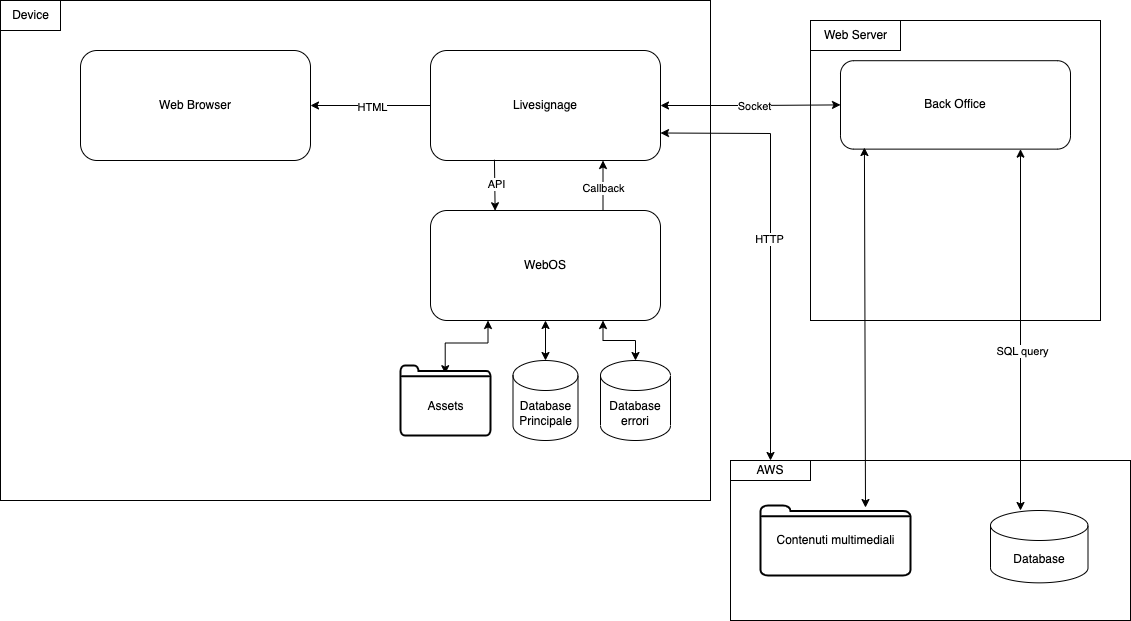
\includegraphics[width= 1\textwidth]{images/svolgimento/webos_client_archi.png} 
    \caption{Architettura del client e dei componenti con cui comunica.} 
    \label{fig:architettura_2}
\end{figure}

\begin{itemize}
    \item Web server: qui vengono salvati in un database MySQL tutte le informazioni degli utenti, dei dispositivi e le playlist create, tutte queste informazioni vengono elaborate e inviate ai client attraverso una socket. Questo si occupa inoltre di caricare su AWS le immagini e i video caricati dal creatore di contenuti in modo da essere scaricabili tramite link dai device client;
    \item Livesignage: dopo aver stabilito il canale di comunicazione con il web server, resta in attesa dei messaggi da questo inviati e si occupa di svolgere le operazioni richieste tramite back office, dal creatore di contenuti, comunicando tramite le API a disposizione, con il sistema operativo sottostante.
    \item Sistema operativo: gestisce le richieste fatte da Livesignage tramite API, una volta che queste sono portate a termine chiama le funzioni di callback passate come parametri dell'API (vedi \ref*{apicode}).
\end{itemize}

Gli altri componenti del sistema sono: il database principale su cui viene salvato il codice HTML delle playlist, il database dei log in cui sono scritti i messaggi di errore in modo che siano successivamente scaricabili dal creatore di contenuti e la cartella degli assets nella quale vengono salvate le immagini e i video delle playlist create in modo che queste possano essere visualizzate anche offline.

\subsection{Codice Livesignage}

\subsubsection{Suddivisione del codice}

Nella cartella principale sono presenti 3 file HTML: 
\begin{itemize}
    \item index.html: è la prima pagina ad essere caricata e si occupa di chiamare le funzioni Javascript per controllare se il device sia stato precedentemente associato a Livesignage.
    \item noAssociation.html: questa pagina viene caricata nel caso che il dispositivo non sia associato e mostra un codice univoco per l'associazione.
    \item display.html: questa è la pagina in cui viene iniettato il codice delle playlist e dei plug-in.
\end{itemize}

Il resto dei file fondamentali si trova nella cartella \jscode{js/}, qui sono raccolti gli script e le classi necessarie al corretto funzionamento dell'applicazione:

\begin{itemize}
    \item association.js: classe che controlla e gestisce l'associazione del device;
    \item connection.js: i metodi di questa classe vengono chiamati ciclicamente per verificare lo stato della connessione;
    \item db.js: classe che si occupa della gestione del database principale, verrà vista in maniera più approfondita ( insieme a dblog.js ) in \ref*{database};
    \item dblog.js: qui è contenuta la gestione del database degli errori;
    \item display.js: in questa classe sono definiti i metodi che implementano la comunicazione con il sistema operativo attraverso le API. Alcune di queste implementazioni verranno approfondite in \ref*{js_code};
    \item filemanager.js: si occupa della gestione del file system del sistema e del download e della cancellazione degli assets;
    \item livesignage.js: in questa classe sono contenuti i metodi per la visualizzazione delle playlist, la gestione di alcuni comandi ricevuti dal server come: il cambio di slide, il passaggio alla visualizzazione dell'ingresso HDMI e le richieste di salvataggio e cancellazione delle playlist dal database;
    \item log.js: qui sono presenti i metodi per la creazione dei messaggi di errore e l'invio di questi al back office in modo che possano essere visualizzati dal cliente;
    \item main.js: questo è lo script principale che si occupa di chiamare le altre classi, in particolare controlla se sia necessario scaricare un aggiornamento dell'applicazione o del firmware del sistema operativo (vedi \ref*{update}), chiama a intervalli di tempo i metodi per il controllo della connessione, invoca i metodi che si occupano della comunicazione con il back office e, se il display risulta offline, avvia la visualizzazione dell'ultima playlist salvata.
    \item monitor.js: questa classe si occupa di aprire la socket verso il back office e di restare in ascolto su questa, alla ricezione dei messaggi chiama i metodi necessari.
    \item speedtest.js: questa classe viene invocata quando si riceve una richiesta per valutare lo stato della rete dal back office.
\end{itemize}

\subsection{Documentazione WebOS Signage}\label{WebOS_doc}

Dopo l'analisi dell'applicazione preesistente è stata studiata la documentazione (disponibile in \cite{LgDoc}) dei dispositivi LG.

Come detto in \ref*{api} sono state analizzate le diverse interfacce messe a disposizone dal sistema per la comunicazione tra il browser e il sistema operativo; le librerie disponibili sono: 
\begin{itemize}
    \item SCAP API: un set di interfacce specifiche per WebOS Signage, la versione di WebOS dedicata ai sistemi di digital signage,suddivise in diverse classi a seconda delle funzionalità. Questo è il set scelto per lo sviluppo poiché, sebbene non sia il più recente, è l'unico compatibile con tutti i device di digital signage di LG e che abbia un set ampio di interfacce tale da coprire i requisiti dell'applicazione;
    \item IDCAP API: è il nuovo standard di API di LG che ha come obiettivo quello di rendere univoche le interfacce per le diverse versioni di WebOS sia quella per il digital signage che quella per le TV commerciali. Nonostante questo set sia quello raccomandato da LG è supportato solamente da WebOS Signage 6.0 e successivi;
    \item Harmony API: una libreria, specifica per WebOS Signage, contenente le interfacce per la comunicazione con alcuni dispositivi esterni come ad esempio stampanti, sensori NFC e infrarossi;
    \item CustomJS API: questo set aggiunge alcune interfacce mancanti alla libreria SCAP. Questa libreria è aggiunta all'applicazione sviluppata al fine di espanderne le funzionalità (si veda \ref*{aggiunte}).
\end{itemize}

Sono state anche studiate le caratteristiche hardware e software dei dispositivi cercando di capire quali fossero quelle minime comuni a tutti. Dal momento che le componenti software e hardware sono molto diverse tra loro a seconda della versione del sistema operativo, sono stati presi in considerazione solo i dispositivi che supportano almeno WebOS signage 4.0. Di seguito sono riportate le specifiche e le versioni dei linguaggi di programmazione supportate che sono state identificate dopo l'analisi.

\begin{center}
\begin{tabular}{ |l|r| } 
     \hline
     HTML & versione 5 \\ 
     CSS & versione 3 \\ 
     JavaScript & versione 1.6+ \\ 
     \hline
     Web Engine & Chrome 53 \\ 
     HTTP, HTTPS & \checkmark \\ 
     XMLHttpRequest (AJAX) & \checkmark \\ 
     JSON & \checkmark \\ 
     \hline
     RAM & 2.0 GB \\
     Memoria & 8.0 GB\\
     Risoluzione & 1920x1080\\
     \hline
\end{tabular}
\end{center}

\section{Scrittura delle classi JavaScript}\label{js_code}

\subsection{Codice delle chiamate alle API} \label{apicode}
Le chiamate API per i dispositivi LG sono di due tipi, le prime ( Listing \ref*{lst:apiget} ) servono per chiedere delle informazioni al sistema operativo come ad esempio il numero seriale, il MAC address o il livello del volume, le seconde (Listing \ref*{lst:apipost}) servono per modificare delle impostazioni di sistema come il volume, lo stato del dispositivo (accensione e spegnimento) o la rotazione dello schermo. In entrambi i casi vengono passate due funzioni dette di callback che saranno eseguite in caso di successo o fallimento della chiamata, le chiamate di modifica del device necessitano inoltre di una struttura contenente i nuovi valori da impostare.

In risposta viene passato un oggetto alle funzioni di callback, in listing \ref*{lst:returnsample} vengono mostrati due esempi: uno in caso di successo, uno di fallimento.

\lstinputlisting[caption={Esempio chiamata API WebOS.}, label={lst:apiget}, language=JavaScript, firstline=0, lastline=18]{listings/svolgimento/api_sample.js}
\lstinputlisting[caption={Esempio chiamata API WebOS.}, label={lst:apipost}, language=JavaScript, firstline=37, lastline=54]{listings/svolgimento/api_sample.js}
\lstinputlisting[caption={Esempi dei messaggi di risposta.}, label={lst:returnsample}, language=JavaScript, firstline=20, lastline=34]{listings/svolgimento/api_sample.js}

Poichè queste funzioni sono asincrone e quindi indipendenti dalla normale esecuzione del codice, è stato necessario gestire l'attesa delle risposte e la sincronizzazione con il resto del codice.

\edit{Javascript non è un linguaggio multi-trhead ma può gestire delle funzioni asincrone tramite un call stack e un event loop che sono parte dell'ambiente di esecuizione JavaScript del browser: il call stack mantiene una coda di tutte le chiamate effettuate dal thread principale, l'event loop si occupa di prendere dalla coda ed eseguire le chiamate asincrone in un ambiente separato dal thread principale, spesso queste funzioni sono interfacce a metodi di basso livello implementati dal web engine in C o C++. In questo modo la funzione successiva nella coda può essere eseguita mentre quella bloccante è eseguita in background. Alle funzioni asincrone possono essere passate come parametri delle funzioni di callback: dei metodi che saranno inseriti nel call stack dall'event loop al termine della funzione bloccante, i parametri di queste funzioni saranno i dati richiesti e l'esito di quanto avvenuto. \cite{MdN}.}

Si è cercato di ridurre il numero di chiamate alle API, per diminuire in maniera sostanziale i ritardi causati da queste, salvando i dati destinati a perdurare nel tempo nel \jscode{localStorage}: un oggetto definito dal browser che permette di salvare in maniera temporanea delle coppie di oggetti chiave-valore. Tuttavia, non essendo assicurata dal browser la persistenza di questo oggetto sono stati implementati tutti i controlli necessari. In \ref*{freestorage} saranno evidenziati i problemi relativi alla capacità del localStorage e alle soluzioni trovate al fine di bilanciare la velocità di esecuzione e la disponibilità dello spazio di memoria.

\subsection{Flusso principale}\label{flusso_principale}

La prima funzione invocata al momento dell'avvio è \jscode{start()} definita in \jscode{main.js} che, come prima cosa controlla se sia disponibile un aggiornamento dell'applicazione o del firmware. Una volta scaricata la nuova versione, dopo aver riavviato il dispositivo, la installa; in caso non siano presenti aggiornamenti o il download non sia riuscito, viene inviata una richiesta al server per verificare se il display sia già stato associato o meno. In caso affermativo, riceve le informazioni relative al contenuto da mostrare, altrimenti viene generato dall'applicazione client \edit{un codice alfanumerico che identifica il display; questo codice sarà poi inserito dal proprietario del display nel portale online in modo da associarvi il device}. Nel caso in cui il display risulti offline all'avvio viene controllato quale sia l'ultimo contenuto salvato sul database e, se disponibile, viene mostrato fino a che non sia possibile collegarsi con il web server e ricevere eventuali nuovi contenuti.


Viene inoltre avviato il controllo a \edit{ intervalli di tempo prestabiliti}, mediante la funzione built-in \jscode{setInterval}, della connessione (Listing \ref*{lst:checkconnection}): viene inviata una richiesta tramite il protocollo HTTP a un URL predefinito e si controlla che questa vada a buon fine (vedi \ref*{connection}).

\lstinputlisting[caption={Controllo dello stato della connesione.}, label={lst:checkconnection}, language=JavaScript]{listings/svolgimento/checkconnection.js}

\section{Cambiamenti di logiche e scelte implementative}

\subsection{Protocollo di comunicazione e gestione della connessione}\label{connection}

\edit{Durante il flusso principale viene mantenuta aperta una socket di comunicazione con il web server: su questa vengono ricevuti i messaggi da parte del back office in caso di cambiamenti ai contenuti da mostrare o alle impostazioni del device sia che siano selezionate direttamente dal creatore di contenuti sia se siano dovute ad automazioni predefinite dall'applicazione. Ad esempio è possibile impostare il cambiamento della playlist in base all'orario o al meteo.}

La classe \jscode{Monitor} si occupa della gestione della socket e all'arrivo di un messaggio chiama le funzioni da eseguire per portare a termine l'operazione richiesta: in Listing \ref*{lst:monitor} viene mostrata una visione parziale della funzione \jscode{parseMessagge()} che si occupa di tutta la gestione.

\lstinputlisting[caption={parseMessage().}, label={lst:monitor}, language=JavaScript]{listings/svolgimento/monitor.js}

Nel caso in cui la socket venga chiusa o a causa di errori o per mancanza di connessione il device viene ritenuto offline: si provvede quindi a eliminare momentaneamente i contenuti che necessitano di una connessione attiva ( meteo, notizie, video online) e viene avviato un meccanismo che prova a riaprire la socket ad intervalli di tempo prestabiliti.
A seguito dei test è stato notato che questo protocollo non assicura di accorgersi in maniera tempestiva dell'assenza di rete ed è stato quindi necessario implementare un secondo protocollo, mostrato in \ref*{flusso_principale}, in cui periodicamente viene fatta una chiamata HTTP per controllare che sia presente la connessione.

La necessità di accorgersi velocemente della mancanza di connessione è dovuta alla presenza delle fonti esterne citate sopra che, qualora non abbiano accesso alla rete, possono mostrare errori, dati non aggiornati o addirittura bloccare l'esecuzione dell'applicazione.

\subsection{Lettura e scrittura dei database} \label{database}

Al fine di garantire che anche in caso di assenza di connessione e ridurre il numero di chiamate HTTP e conseguenti download degli assets necessari, all'arrivo dei dati dal back office: al momento del cambio di una playlist o dell'inserimento di un plug-in, tutti i dati sono salvati in locale su un database non relazionale.

\edit{Dal momento che JavaScript non prevede i metodi per la comunicazione con un database SQL}, è stata usata la libreria Dixie.js \cite{dixie} che permette di salvare i dati necessari in un file di testo, appositamente formattato, e accederli tramite indicizzazione chiave - valore. Il file viene letto all'avvio dell'applicazione e viene creato il database che sarà quindi accessibile tramite le funzioni della libreria. Il salvataggio del database avviene sovrascrivendo il vecchio file nel file system.

Dixie.js si occupa di creare e leggere le entry nell'\jscode{IndexedDB}: un database NoSQL presente nel web browser. Come il \jscode{localStorage} (vedi \ref*{freestorage}) questo database non assicura la persistenza dei dati ma è pensato, a differenza del primo, per ospitare una grande quantità di dati. La libreria, oltre a facilitare le operazioni di lettura e scrittura, permette di ricreare velocemente la struttura e i dati contenuti nel database al momento dell'ultimo salvataggio.

Durante lo studio della documentazione LG è stato osservato che il buffer di memoria per la lettura e scrittura di un file è solo di 10 KB; è stato quindi necessario implementare le funzioni di scrittura e lettura di un file in maniera ricorsiva in modo che fosse possibile usarla come funzione di callback.
Dal momento che il numero di chiamate necessarie a portare a termine le operazioni è elevato ed i tempi di esecuzione intorno ai 30s, è stato quindi deciso di implementare le due funzioni in modo completamente asincrono rispetto al resto del flusso di esecuzione. 

Nonostante questo, il carico di lavoro risulta piuttosto elevato e di conseguenza i rallentamenti dei contenuti mostrati sono comunque evidenti soprattutto durante la scrittura del database. 

\lstinputlisting[caption={Scrittura ricorsiva del database.}, label={lst:dbwrite}, language=JavaScript]{listings/svolgimento/databasewrite.js}

Nel Listing \ref*{lst:dbwrite} sono mostrate le due funzioni usate per la scrittura del database; inizialmente viene eliminato il file precedentemente salvato e, in caso di successo, prima viene fatto un encoding in bytes della stringa rappresentante il contenuto del file e successivamente la funzione di \jscode{doStoreFile()} scrive 10KB alla volta sul file.

Sono state pensate diverse soluzioni possibili, tra le quali: il salvataggio di un minor numero di dati, la suddivisione in database distinti per gli assets e il codice delle playlist o la cancellazione periodica dei dati più vecchi. Al momento nessuna di queste opzioni è risultata applicabile o per motivi legati alla struttura del database o per mantenibilità rispetto agli altri client.

\subsection{Cancellazione del localStorage} \label{freestorage}

Il \jscode{localStorage} è un database formato da coppie chiave-valore presente direttamente sul web browser. Questo database è pensato per mantenere una piccola quantità di dati che devono essere disponibili a pagine HTML diverse, ma sempre nello stesso dominio, anche dopo aver eseguito il refresh. Nonostante i dati possano essere mantenuti in memoria anche tra diverse sessioni, la persistenza non è garantita.  

Nell'applicazione le informazioni relative alle playlist e ai plug-in vengono salvate, oltre che sul database, anche nel \jscode{localStorage}; in questo modo vengono ridotti i tempi di accesso al dato, dovendo leggere le informazioni sul database solo in caso non siano presenti nel \jscode{localStorage}.

In seguito ai test è stato osservato che la memoria disponibile nel \jscode{localStorage} è limitata, intorno ai 5 MB per l'insieme di tutti i dati salvati e molto minore per la singola entry, ed è stato quindi necessario gestire tutte le scritture e le conseguenti cancellazioni dei dati salvati in questa struttura. Al fine di mantenere libera la memoria del dispositivo, di non aumentare il numero delle chiamate al web server e i tempi di esecuzione al momento del cambio di contenuto, è stato fatto in modo che solo i dati necessari a quanto programmato restino salvati nel localStorage per permettere un rapido accesso e vengano cancellati al momento del cambio del contenuto. In questa esecuzione è stata prestata particolare attenzione nel mantenere i dati relativi alle immagini e video precedentemente scaricati e al caso in cui una playlist venga solo aggiornata e non ci sia quindi bisogno di scaricare nuovamente tutto il contenuto.

\subsection{Aggiornamento del firmware di sistema e dell'applicazione}\label{update}

Rispetto agli altri client una delle API, messe a disposizione dal sistema, permette di scaricare e aggiornare il firmware del sistema operativo a partire da un URL che punti al file di aggiornamento.
È stata quindi aggiunta la possibilità di inviare un messaggio, tramite la socket, al sistema contenente l'URL della nuova versione. L'applicazione si occuperà quindi di scaricare e installare l'aggiornamento o, in caso di errore, mantenere la versione attuale senza la perdita di informazioni.

Di seguito è riportata la funzione che si occupa del download e dell'aggiornamento del firmware.

\lstinputlisting[caption={Aggiornamento del firmware.}, label={lst:fwupd}, language=JavaScript]{listings/svolgimento/firmware_update.js}

Ad ogni avvio viene inoltre controllato se l'applicazione deve essere aggiornata.
Come mostrato in Listing \ref*{lst:updls} per prima cosa si imposta un time-out in modo da dare il tempo al device di stabilire la connessione a internet, successivamente viene fatta una chiamata alle API del backoffice per controllare quale sia la versione online corrente dell'applicazione e, nel caso questa differisca da quella installata al momento, viene scaricata e installata.

\lstinputlisting[caption={Aggiornamento applicazione.}, label={lst:updls}, language=JavaScript]{listings/svolgimento/upd_ls.js}

Anche in questo caso una copia del file dell'applicazione attuale viene mantenuta in memoria fino al momento dell'aggiornamento, in modo che il client possa funzionare in caso di errore.

\subsection{Gestione input del telecomando}

Un'altra importante funzionalità aggiunta è stata quella di poter cambiare la gestione dei segnali ricevuti dal telecomando  all'interno dell'applicazione.
Questo, oltre a evitare che persone non autorizzate possano interagire con il display, permette di personalizzare l'esperienza utente e le funzionalità dell'applicazione senza la necessità di passare dal back office.

In WebOS è presente una tabella (una versione semplificata è mostrata nella Tabella \ref*{tab:keycode}) dove sono indicati tutti i codici che un telecomando può inviare, la stringa che questi rappresentano e un valore che identifica se deve essere gestito dal sistema o dall'applicazione.

\begin{table}
    \centering
    \begin{tabular}{ |c|c|c| } 
         \hline
         409 & Signage.KeyCode.POWER & 0 \\  
         \hline
         461 & Signage.KeyCode.BACK & 0 \\  
         \hline
         601 & Signage.KeyCode.EXIT & 0 \\  
         \hline
         ... & ... & ...\\
         \hline
    \end{tabular}
    \caption{Codici telecomando} \label{tab:keycode}
\end{table}
    
Per modificare la funzione di un segnale è quindi necessario inserire nella tabella che questo sarà gestito dall'applicazione e successivamente indicare quale azione eseguire. In Listing \ref*{lst:setkey} è mostrata la funzione che si occupa di cambiare il dato nella tabella e in Listing \ref*{lst:getkey} viene mostrato come alla ricezione di un segnale, in questo caso \jscode{Signage.KeyCode.RIGHT_ARROW}, venga eseguita una funzione specifica.

\lstinputlisting[caption={Modifica tabella comandi.}, label={lst:setkey}, language=JavaScript, firstline=0, lastline=19]{listings/svolgimento/keycode.js}
\lstinputlisting[caption={Ricezione di un segnale.}, label={lst:getkey}, language=JavaScript, firstline=20, lastline=49]{listings/svolgimento/keycode.js}

In alcuni casi, ad esempio il segnale di spegnimento, il comando viene prima gestito dall'applicazione e successivamente inviato al sistema. Questo permette di avere il controllo di alcuni momenti critici, come l'uscita dall'applicazione, per poter salvare i dati necessari o inviare i dati per le statistiche.
In Listing \ref*{lst:keysys} viene mostrata la chiamata che si occupa di inviare il segnale al sistema.

\lstinputlisting[caption={Invio di un segnale al sistema.}, label={lst:keysys}, language=JavaScript, firstline=50, lastline=70]{listings/svolgimento/keycode.js}

I comandi che rientrano in questo caso sono stati ridotti al minimo e si è cercato di rendere il tempo di esecuzione il più breve possibile al fine di mantenere un'esperienza utente coerente.

\section{Fase di testing}

La fase di test è stata suddivisa in due momenti: inizialmente sono state testate le singole funzionalità durante la scrittura dell'applicazione e successivamente sono stati svolti una serie di test, in maniera più approfondita, di tutto il sistema.

La prima fase ha evidenziato molti dei problemi descritti precedentemente, dando quindi la possibilità di analizzarli e trovare soluzioni alternative.
Nella seconda fase ci si è cercato di capire quali fossero i limiti, dovuti all'hardware e al software a disposizione:
\begin{itemize}
    \item Stress test: sono state inserite una serie di playlist contenenti un alto numero di slides di diverso tipo in modo da capire i tempi necessari al download, di scrittura del database e la reattività nel cambio tra le slide;
    \item Test sulla rete: sono state testati i tempi entro cui il device si accorge dell'assenza di rete e delle tempistiche necessarie ad eliminare i contenuti non disponibili offline;
    \item Test del web engine: sono state inserite diverse slide il cui contenuto potesse risultare difficile da gestire per il browser e playlist composte da 4 playlist mostrate contemporaneamente.
\end{itemize}

\edit{Tutti i test sono stati svolti su entrambi i dispositivi a disposizione: è stato notato che il media player si è dimostrato migliore per quanto riguarda la velocità di scrittura del file del database nel file system mentre il display riesce a gestire i maniera più fluida i contenuti da mostrare in particolare quando questi presentano molte animazioni o un alto numero di componenti.}

\edit{In generale i dispositivi LG si sono dimostrati meno performanti rispetto a quelli Samsung (su cui era già disponibile Livesignage) ma hanno alcune caratteristiche uniche come la possibilità di mostrare fino a 4 video contemporaneamente e la maggiore compatibilità con le periferiche esterne (si veda \ref*{aggiunte}).}